\section{Discussion}
\footnote{\url{https://github.com/lucasabdalah/Exploratory-Data-Analisys/blob/main/code/hw2/data_regression.ipynb}}

\begin{figure}[htbp!]
  \centerline{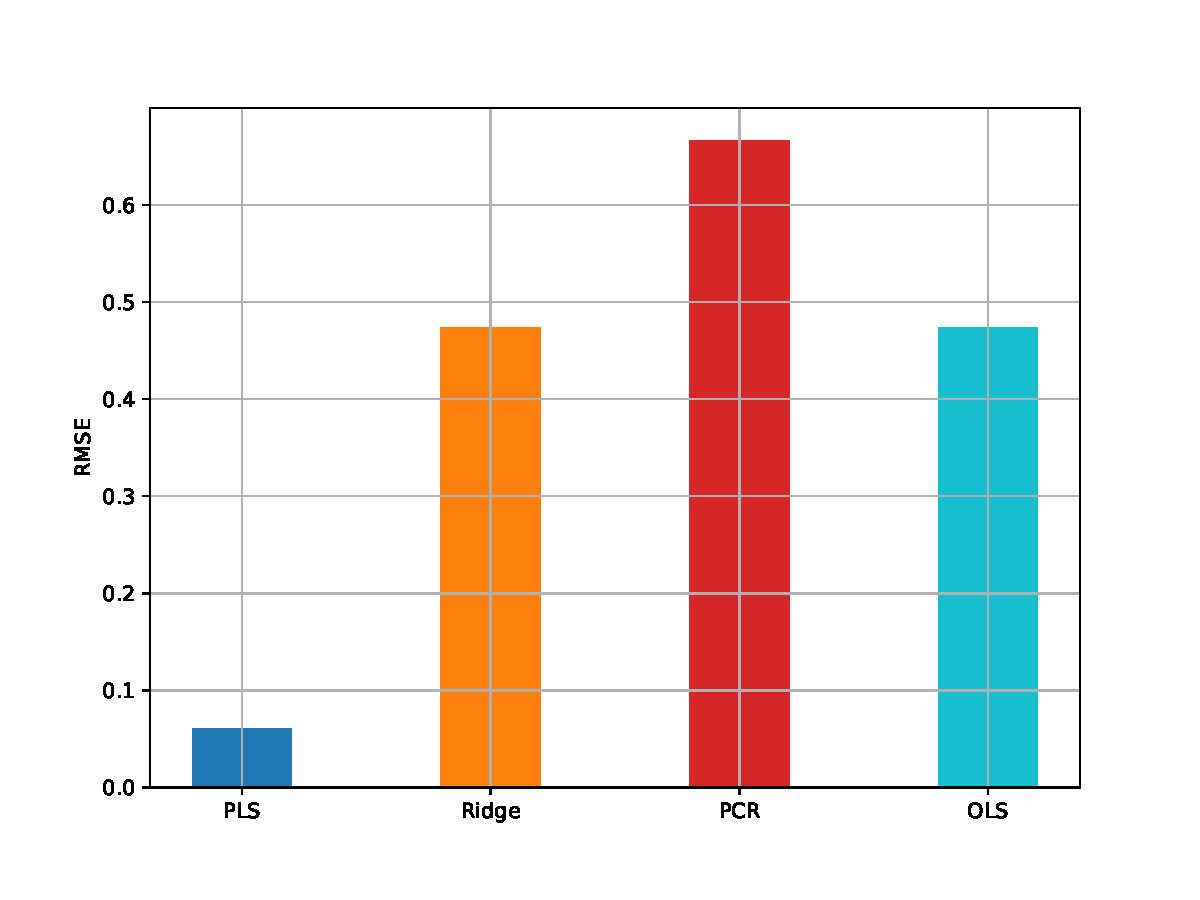
\includegraphics[width=0.5\textwidth]{../../code/hw2/figures/5-summary.pdf}}
  \caption{Best value for RMSE for the proposed approaches.}
  \label{fig:5-summary}
\end{figure}


\section{Conclusion}
Among the results obtained, there were no great differences between the results of the models, which favors the use of simpler models and lower computational cost, to the detriment of little improvement in prediction with the increase of cost. Therefore, unless there is a real need to obtain the best possible results, the most cost-effective solution was simple linear regression, since it is inexpensive and obtained results that were not much inferior to its peers. 

Nonetheless if computational cost is not taking in account, the best model for the given data set is the ridge regression model, since it presented the best results both in validation and in the test set.

% Dentre os resultados obtidos o não foram constatadas grandiosas diferenças dentre os resultados dos modelos, isso favorece a utilização de modelos mais simples e de menor custo computacional, em detrimento da pouca melhora da predição com o aumento do custo. Portanto ao menos que de fato haja uma necessidade em obter o melhor resultado possível, a solução com melhor custo-benefício foi a regressão linear simples, visto que é pouco custosa e obteve resultados não muito inferiores aos seus correntes, mas caso o custo computacional não precise ser considerado, o melhor modelo para o conjunto de dados fornecido é o de regressão ``ridge'', pois esse foi o que obteve os melhores resultados tanto na validação quanto no conjunto de teste.


\section{Further Work}


\section*{Appendix}

\begin{figure}[htbp!]
  \centerline{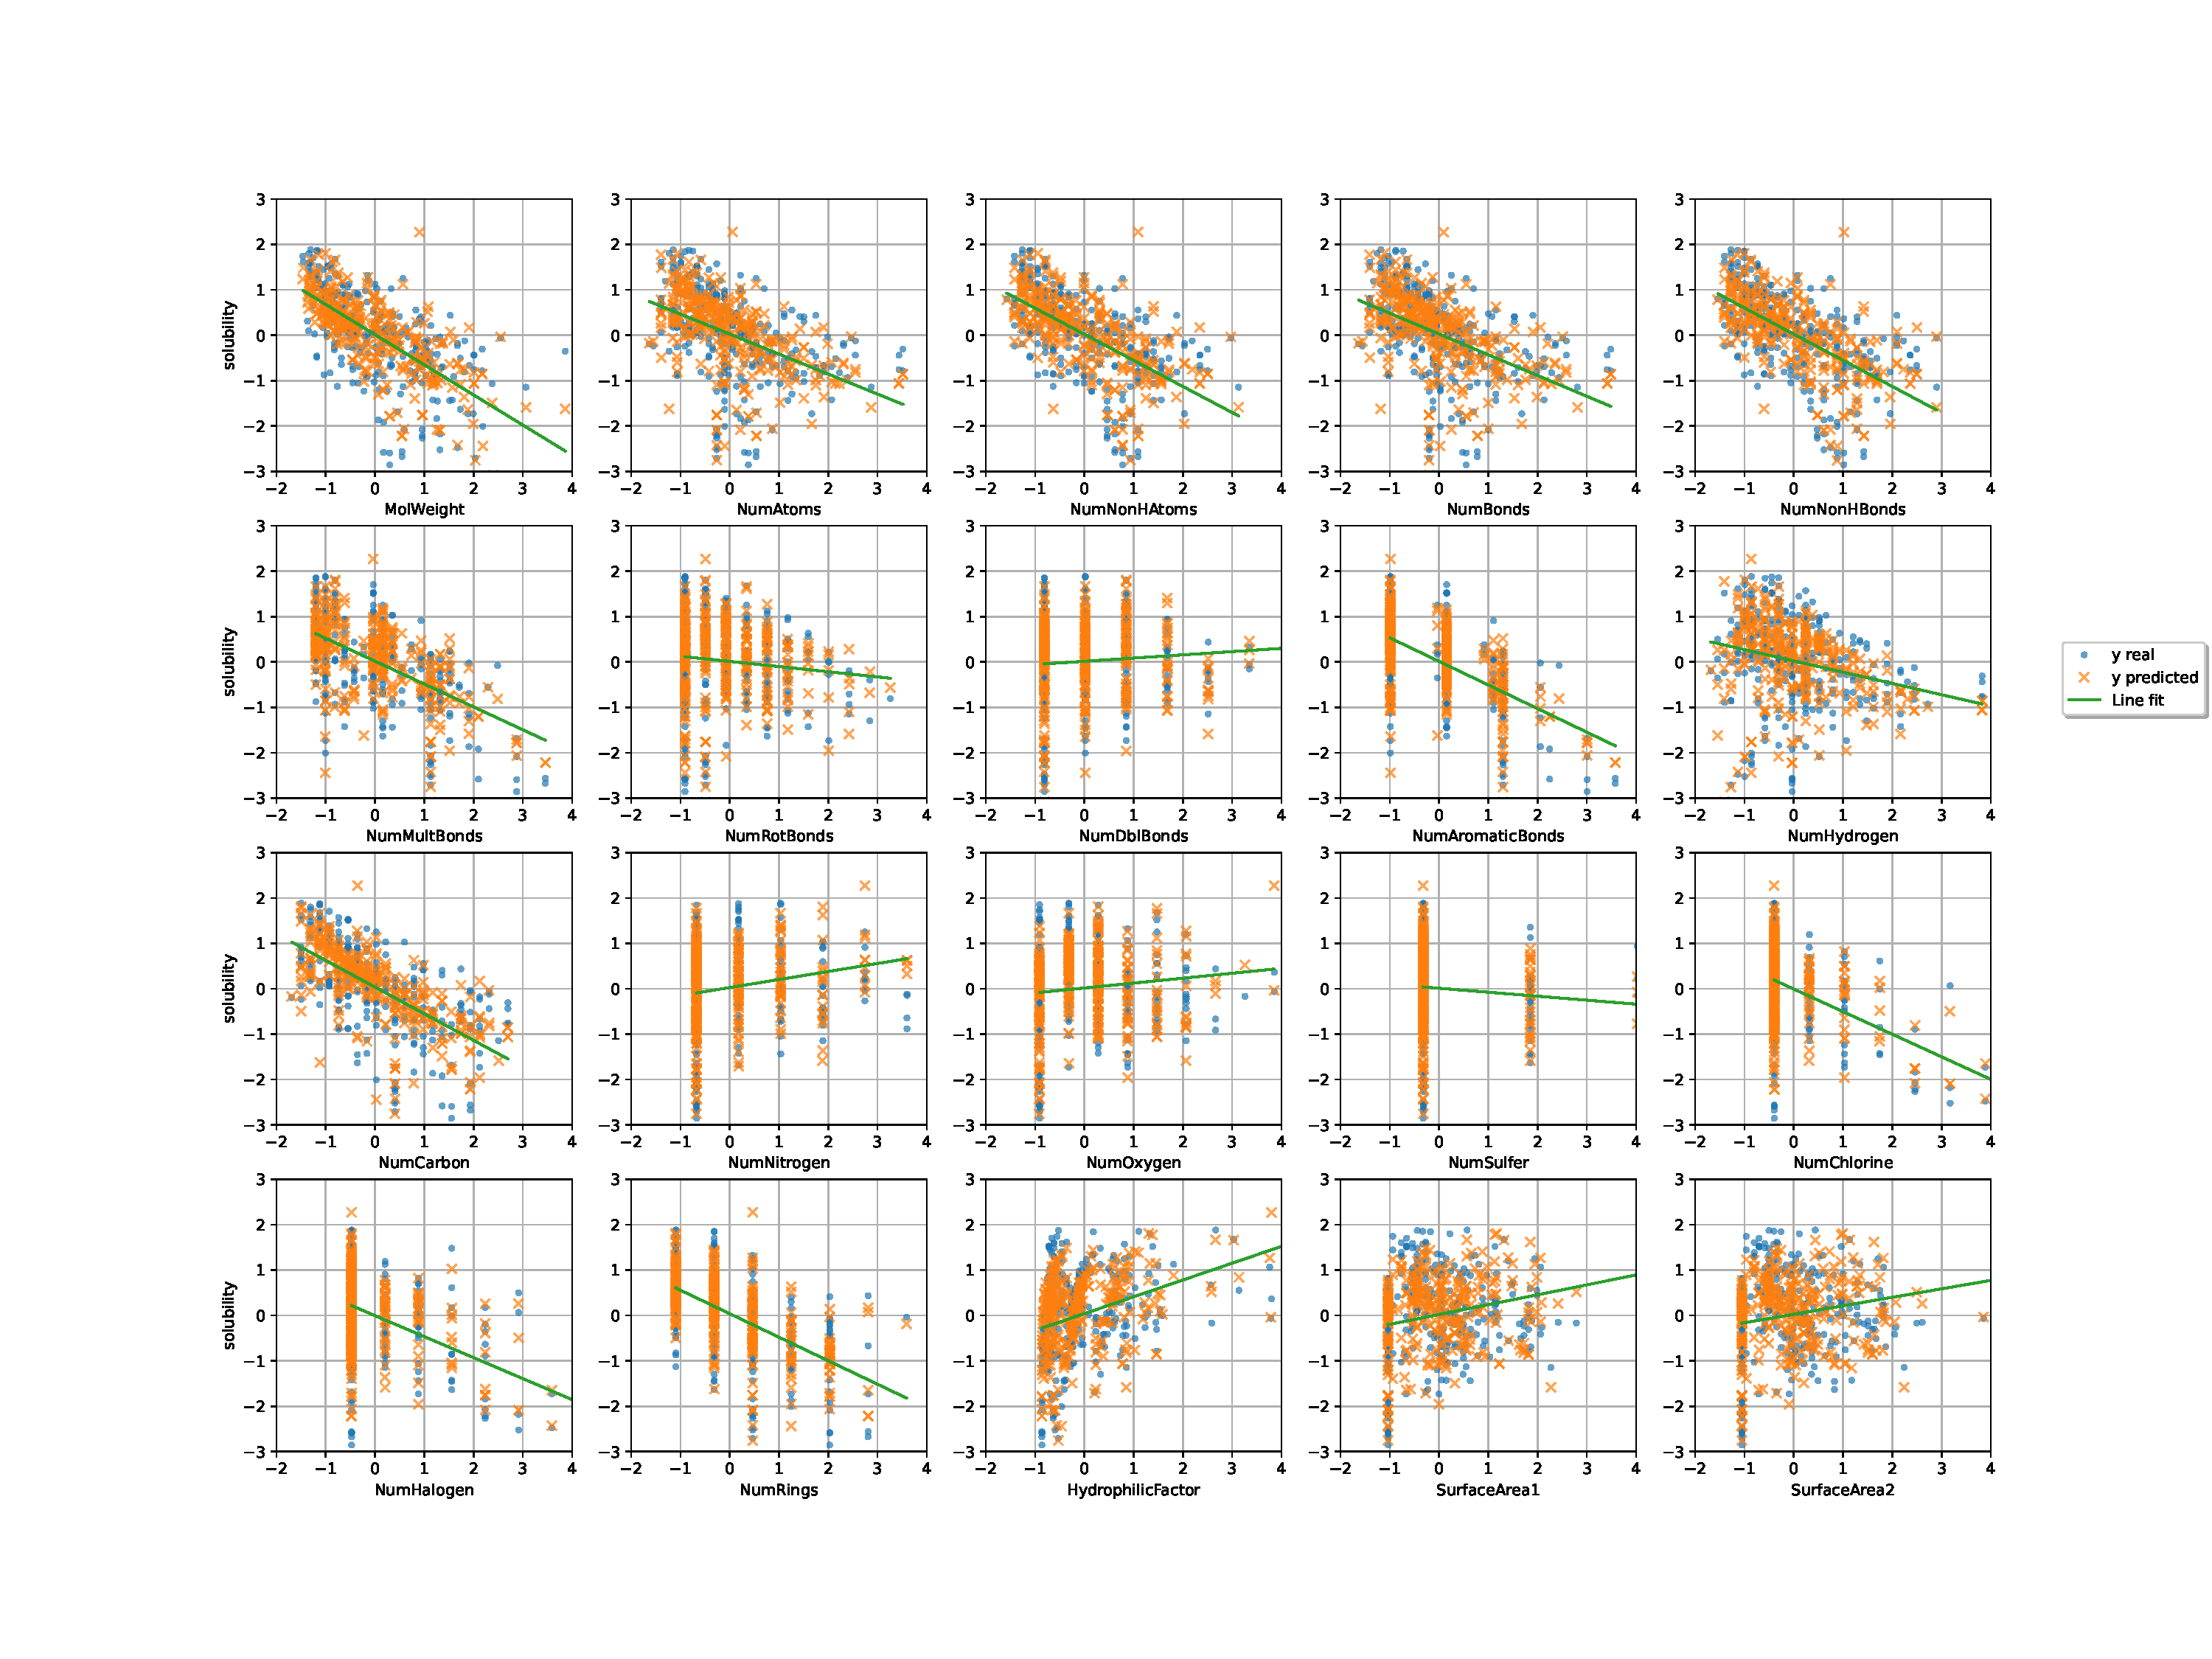
\includegraphics[width=0.6\textwidth]{../../code/hw2/figures/2-linear-regression.pdf}}
  \caption{Linear regression.}
  \label{fig:2-linear-regression}
\end{figure}

